\documentclass[14px]{article}
\usepackage{xeCJK}
\usepackage[frenchb]{babel}
\usepackage[T1]{fontenc}
\usepackage[utf8]{inputenc}
\usepackage{textcomp}
\usepackage{amssymb}
\usepackage[ruled,longend]{algorithm2e}
\usepackage{amsmath}
\usepackage{latexsym}
\usepackage{fancyhdr}
\usepackage{geometry}
\usepackage{setspace}
\usepackage[colorlinks,linkcolor=blue]{hyperref}
% Image
\usepackage{graphicx}
\usepackage{float}
\usepackage{subfigure}
\usepackage{enumerate}

\begin{document}
\setlength{\parindent}{0pt}
\begin{titlepage}
	\begin{center}
		% Upper part of the page
		
\includegraphics[width=0.35\textwidth]{logo.png}\\[1cm]
		\textsc{\Large Rapport de PC3R}\\[0.5cm]
		% Title
		{ \huge \bfseries Système de Gestion de Location}\\[0.4cm]
		% Author and supervisor
		\begin{minipage}{0.4\textwidth}
			\begin{flushleft} \large
				\emph{Author:}\\
				Qiwei \textsc{XIAN}\\
				Ruiwen \textsc{WANG}\\
			\end{flushleft}
		\end{minipage}
		\begin{minipage}{0.4\textwidth}
				\begin{flushright} \large
				\emph{Professeur:} \\
				Prof.\textsc{Romain Demangeon}
			\end{flushright}
		\end{minipage}
		\vfill
		% Bottom of the page
		{\large \today}
	\end{center}
\end{titlepage}
\clearpage

\tableofcontents
\thispagestyle{empty}
\clearpage
\section{Introduction}
Système de gestion de location est une plateforme communautaire de location et de réservation de logements personnels. Les fonctionnalités du système est ressemble à Airbnb. Il permet aux utilisateurs de louer leur propriétés immobilières et de réserver un logement de l'autre utilisateur.

Chaque l'utilisateur doit inscrire sur le système afin d'obtenir un compte, il bénéficie de la service du système en utilisant ce compte. Il peut créer une espace de client et enregistrer les informations publiques, chaque utilisateur peut consulter les informations des autres utilisateurs.

Il peut tourver des logements qui satisfait à ses beosins, par exemple sous la condition de période de location, la ville, le nombre des locataires, ainsi que le droit de fumer.
L'utilisateur peut aussi gérer leur propriétés par ce systèmes, il d'abord ajoute ses logements à louer dans le compte et met les contraintes pour les locataires, par exemple le nombre des locataires ou l'interdiction de fumer, etc.  En plus il peut les modifier ou supprimer comme il veut. Lors que l'utilisateur reçoit les demandes envoyées par les autres utilisateurs. Il a droit de la refuser ou accepter, mais si la demande a risque de causer un conflit, le système va le faire remarquer au propriétaire.

\section{API Web choisie}
\subparagraph{Weatherstack}
Nous utilisons cette API pour aider les utilisateurs à savoir la météo la ville qu'il souhaite réserver.\\
L'API Weatherstack[1] est développée par une société britannique qui excelle en SaaS avec des sociétés comme Ipstack, Currencylayer, Invoicely et Eversign. Destiné principalement aux sites Web et aux applications mobiles qui cherchent à inclure un widget météo en direct à un coût minime, offre la météo en temps réel, la météo historique, la météo internationale, etc.\\
Intégration et format de l'application: l'API REST renvoie des réponses au format JSON et prend en charge les rappels JSONP. HTTPS est activé pour les abonnements payants.\\
Nous enverrons régulièrement les informations contenant la ville qu'utilisateur veut réserver au serveur wheather via l'Api. Puis,l'API REST renvoie des réponses au format JSON à notre serveur Notre serveur reçoit les informations au format JSON et affiche les informations météo sur la page.
\subparagraph{Google Map}
Pour aider les utilisateurs à savoir où se trouvent ces propriétés immobilières,nous utilisons Google Maps pour localiser ces propriétés immobilières.
Google Maps[2] est un service de cartographie en ligne. C'est un service disponible sur PC, sur tablette et sur smartphone qui permet, à partir de l'échelle mondiale, de zoomer jusqu'à l'échelle d'une habitation.\\
En utilisant l'Api Google Maps, on peut intégrer Google Maps sur notre site. Il nous propose une carte sur une interface graphique. Nous enverrons l'adresse de la propriété immobilière au serveur de Google via l'Api google maps. La interface graphique du Google maps sur le site sera localisées en fonction de cette adresse et affichera cette adresse.
\section{Mettre à jour les données}
\subsection{Mettre à jour Weatherstack}
Observons d'abord à quoi ressemblent les données json renvoyées de Weatherstack, comme montré dans Annexe d'image "cf.Données Json".\\
Lorsque l'utilisateur entre dans une page de détail de la propriété immobilière:notre fonction js ajoutera en texture html une fonction \textbf{autoRefreshWheather} pour appeler régulièrement la fonction \textbf{getWheather}\\

\begin{figure}
		\subfigure{
			\begin{minipage}[t]{\linewidth}
				\centering
				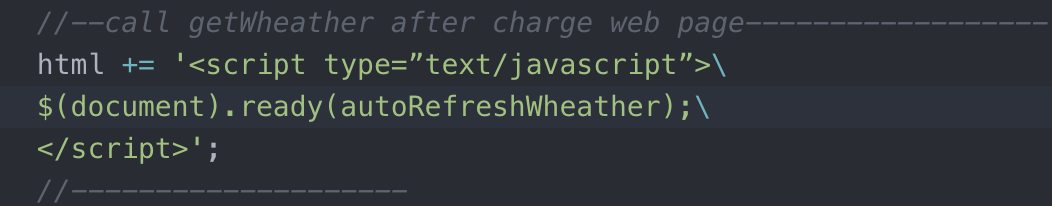
\includegraphics[width=0.8\textwidth]{callAutoRefresh.png}\\
				\caption cf.Données Json
			\end{minipage}%
		}%
\end{figure}

La fonction \textbf{autoRefreshWheather} appelle la fonction \textbf{getWheather} toutes les 5 minutes.\\

\begin{figure}
		\subfigure{
			\begin{minipage}[t]{\linewidth}
				\centering
				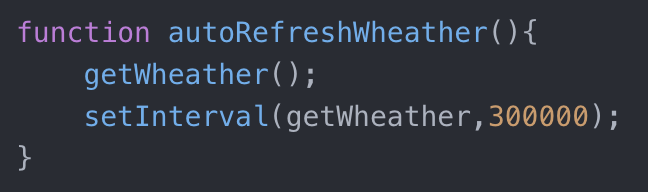
\includegraphics[width=0.8\textwidth]{reFresh.png}\\
				\caption cf.reFresh
			\end{minipage}%
		}%
\end{figure}

La fonction \textbf{getWheather} envoie les informations correspondant à la ville du client au serveur et attend que le serveur renvoie les données json, puis affiche les données json sur html en appelant htmlWheather.

\begin{figure}
		\subfigure{
			\begin{minipage}[t]{\linewidth}
				\centering
				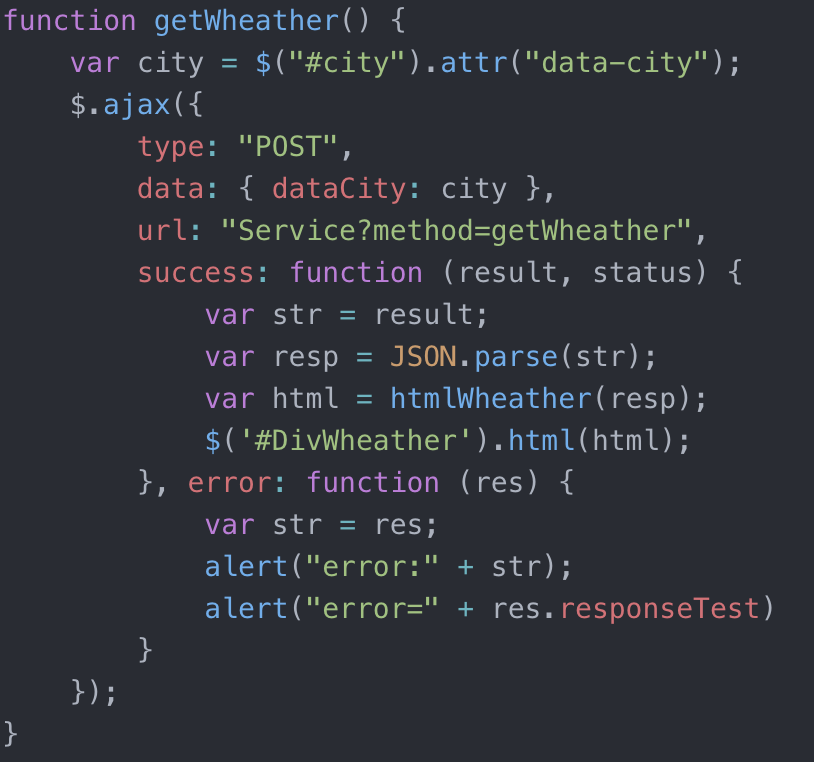
\includegraphics[width=0.8\textwidth]{getWheather.png}\\
				\caption cf.getWheather
			\end{minipage}%
		}%
\end{figure}

Après réception de la demande, le serveur établit une connexion avec le serveur Weatherstack. Le serveur Weatherstack jugera s'il faut accepter la demande en fonction de la clé d'accès et retournera les données json en fonction de la valeur de la requête après avoir accepté la demande. Le serveur renvoie ensuite les données json au client via la méthode resp.getWriter().Write.\\

\begin{figure}
		\subfigure{
			\begin{minipage}[t]{\linewidth}
				\centering
				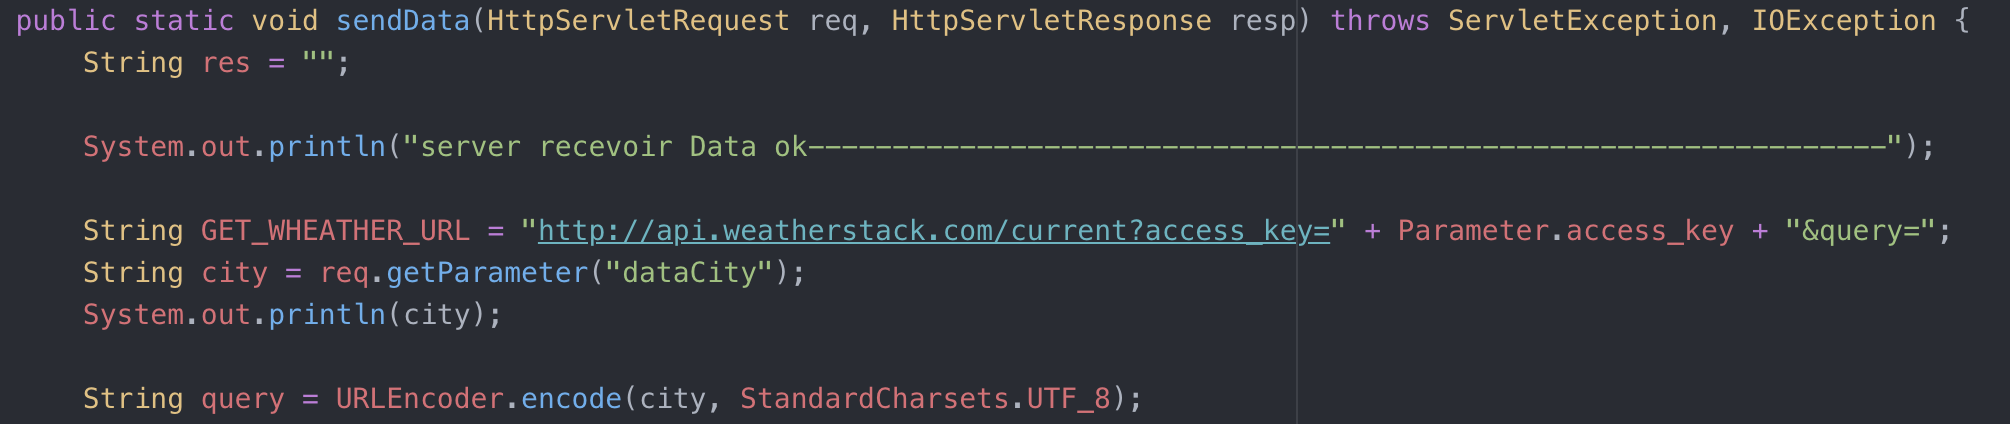
\includegraphics[width=1\textwidth]{setupConnection.png}\\
				\caption cf.setupConnection
			\end{minipage}%
		}%
\end{figure}

Enfin, nous afficherons les résultats des données json sur html.

\begin{figure}
		\subfigure{
			\begin{minipage}[t]{\linewidth}
				\centering
				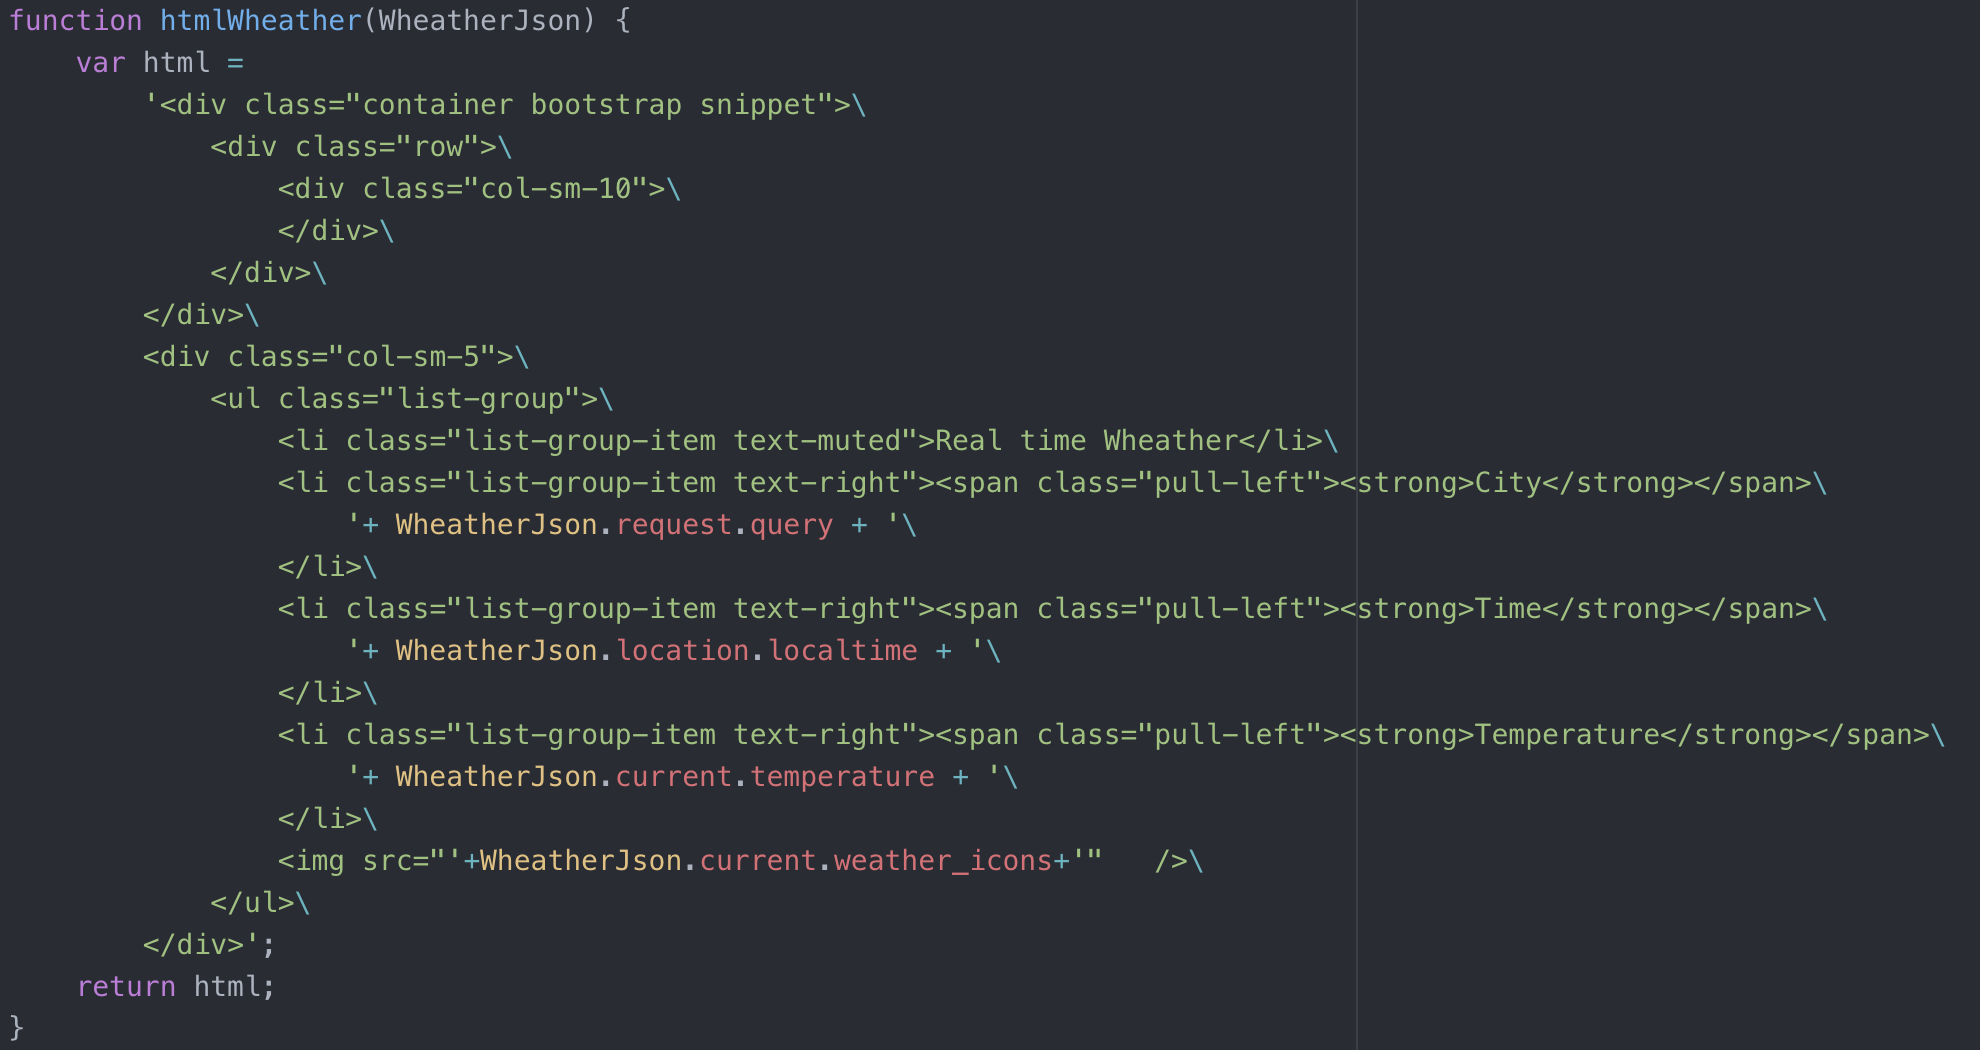
\includegraphics[width=1\textwidth]{htmlWheather.png}\\
				\caption cf.htmlWheather
			\end{minipage}%
		}%
\end{figure}

\subsection{Mettre à jour Google Map}
Chaque fois ,l'utilisateur entre dans une page de détail de la propriété immobilière,	nous appellerons Google Maps pour localiser
la propriété immobilière.Le lien ci-dessous \textbf{googleapis} appellera en façon callback la méthode de js :\textbf{initMap}.
Il est à noter que le mot-clé \textbf{asyns} peut réaliser un chargement asynchrone, ce qui signifie que ce lien sera appelé après le chargement du HTML

\begin{figure}
		\subfigure{
			\begin{minipage}[t]{\linewidth}
				\centering
				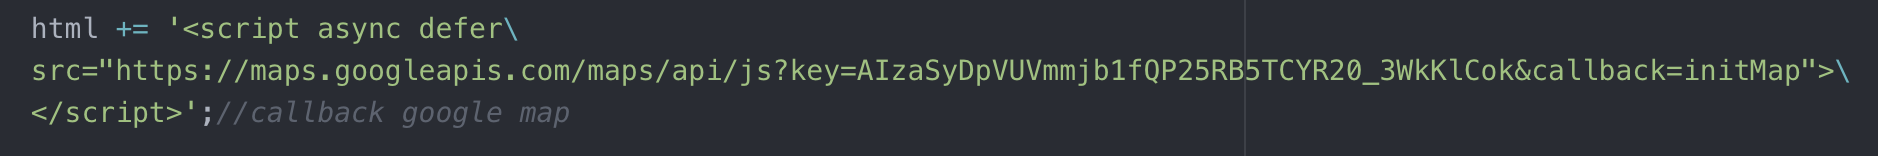
\includegraphics[width=1\textwidth]{htmlGoogleMaps.png}\\
				\caption cf.htmlWheather
			\end{minipage}%
		}%
\end{figure}

Les fonctions initMap et geocodeAddress permettent à Google Maps de s'initialiser en fonction du lieu donné.

\begin{figure}
		\subfigure{
			\begin{minipage}[t]{\linewidth}
				\centering
				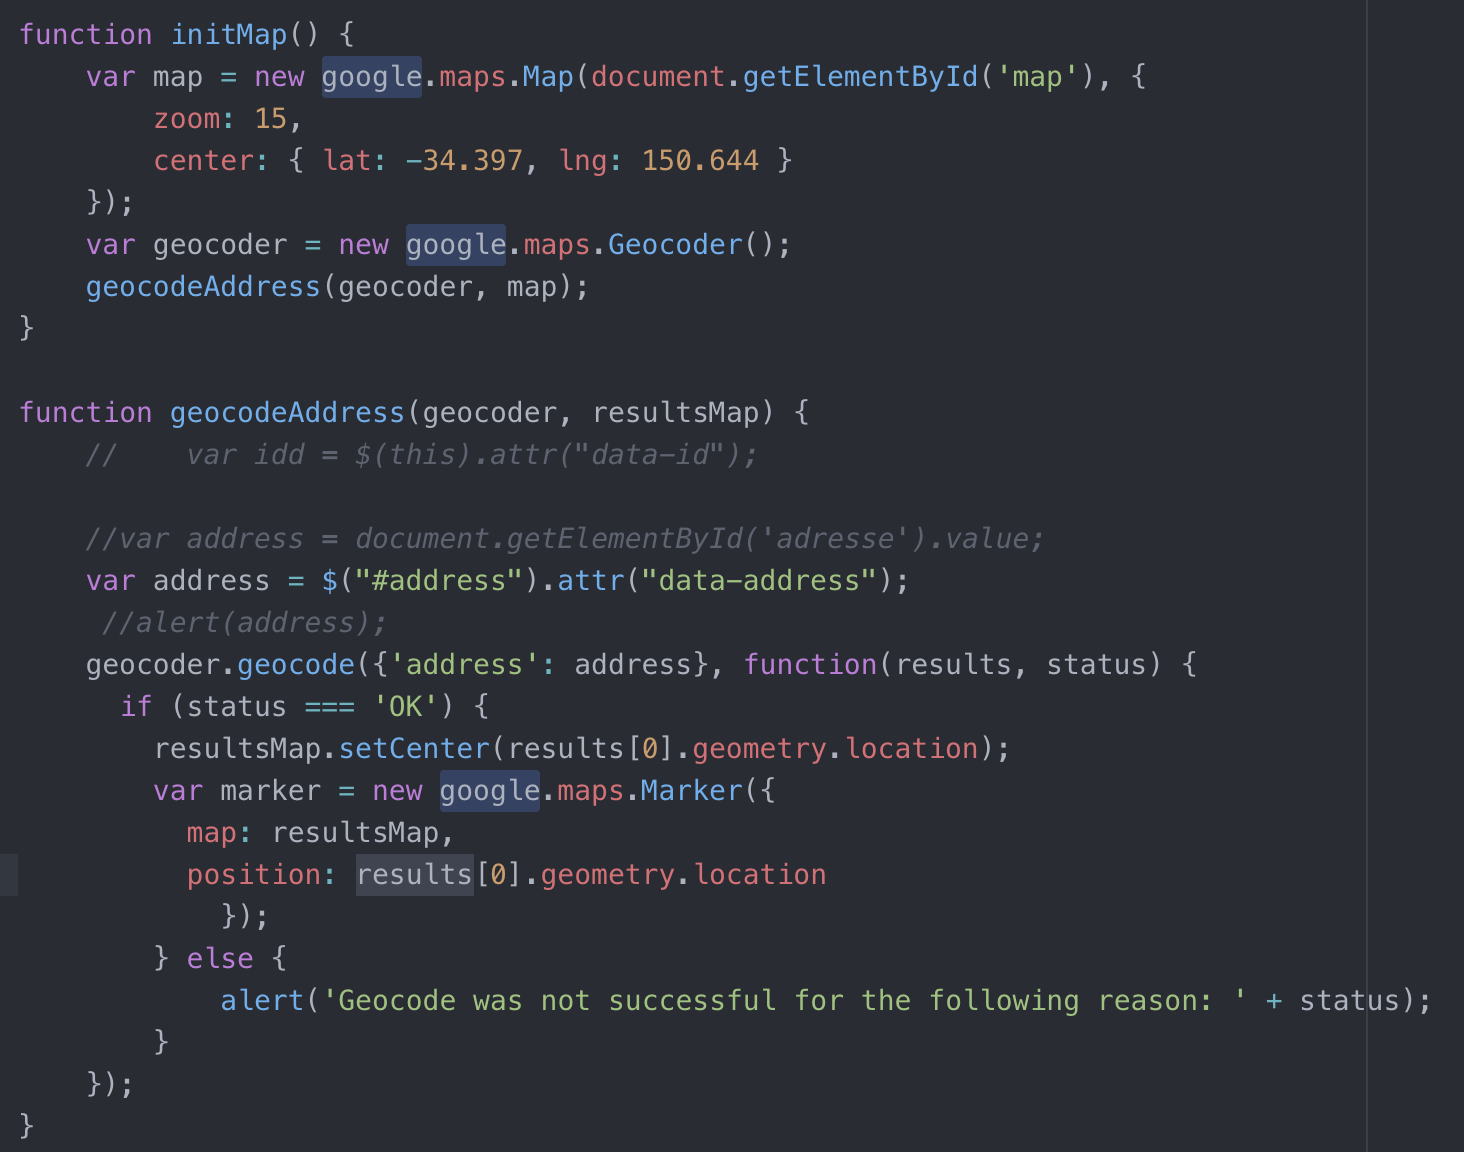
\includegraphics[width=1\textwidth]{initMaps.png}\\
				\caption cf.initMaps
			\end{minipage}%
		}%
\end{figure}


\section{Fonctionnalités}
Le système est séparer en trois modules, \textbf{compte}, \textbf{demande}, \textbf{propriété}. Cela permet de faciliter le développement et la maintenance de l'application. On a réaliser les fonctionnalités de l'ajoute, de la suppression et de la consultation, ainsi que la modification de ces trois modules.

\section{Cas d'utilisations}
\subsection{Inscription}
Acteur : L'utilisateur\\
Contexte : L'utilisateur crée un compte.\\
Scénario principal:
\begin{enumerate}
	\item L'utilisateur entre dans le page d'inscription.
	\item L'utilisateur saisit l'identifiant et le mot de passe.
	\item L'utilisateur clique Signup pour soumettre les information au serveur.
	\item Le système répond le message de success et afficher sur l'écran.
\end{enumerate}
Cas particulier:\\
4a. L'identifiant est déjà utilisé dans le système, le système affiche le message d'erreur.

\subsection{Authentification}
Acteur: L'utilisateur\\
Contexte: L'utilisateur s'authentifie dans le système par son compte.
Scénario principal:
\begin{enumerate}
	\item L'utilisateur entre dans le page de l'authentification.
	\item L'utilisateur saisit l'identifiant et le mot de passe.
	\item L'utilisateur clique le button Login pour soumettre les informations au serveur.
	\item Le serveur vérifie l'identifiant et le mot de passe.
	\item Le serveur rend le page web de \textbf{mainPage.jsp}, l'identifiant est stocké dans la session.
\end{enumerate}
Cas particulier: \\
4a. L'identifiant n'est pas reconnu, le système affiche le message d'erreur.\\
4b. Le mot de passe n'est pas correspondant à l'identifiant, le système affiche le message d'erreur.

\subsection{Consulter l'espace du client}
Acteur: L'utilisateur\\
Contexte: L'utilisateur connecté veut consulter son espace du client.
Scénario principal:
\begin{enumerate}
	\item L'utilisateur clique le button Profile dans mainPage.
	\item Le serveur génère dynamiquement l'espace personnelle de l'utilisateur.
\end{enumerate}
cas particulier:\\
2a. L'utilisateur n'a pas encore son espace du client, le serveur génère le page de creation d'espace, permet à l'utilisateur de créer son espace.


\subsection{Créer l'espace du client}
Acteur: L'utilisateur\\
Contexte: L'utilisateur consulte sont espace première fois
Scénario principal:
\begin{enumerate}
	\item L'utilisateur clique le button Profile première fois dans le mainPage.
	\item Le serveur repond un message et génère dynamiquement le formulaire pour créer l'espace du client.
	\item L'utilisateur saisit les informations publiques.
	\item L'utilisateur clique le button Créer afin de soumettre les information.
	\item Le serveur crée l'espace du client et le stocke dans la base de données, ainsi que génère le page web de l'espace du client.
\end{enumerate}

\subsection{Modifier l'espace du client}
Acteur: L'utilisateur
Contexte: L'utilisateur connecté se trouve dans le mainPage.
Scénario principal:
\begin{enumerate}
	\item L'utilisateur clique le button Profile
	\item Le serveur
\end{enumerate}




\section{Stockage des données}
Les données sont stockées dans la base de données SQL,avec 4 quatre tables, la structure de ces 4 tables est comme indiqué ci-dessous.\\
\begin{figure}
		\subfigure{
			\begin{minipage}[t]{\linewidth}
				\centering
				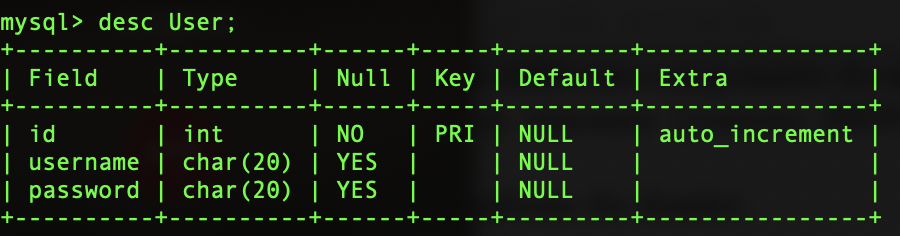
\includegraphics[width=0.5\textwidth]{tableUser.png}\\
				\caption cf.tableUser
			\end{minipage}%
		}%
\end{figure}
\begin{figure}
		\subfigure{
			\begin{minipage}[t]{\linewidth}
				\centering
				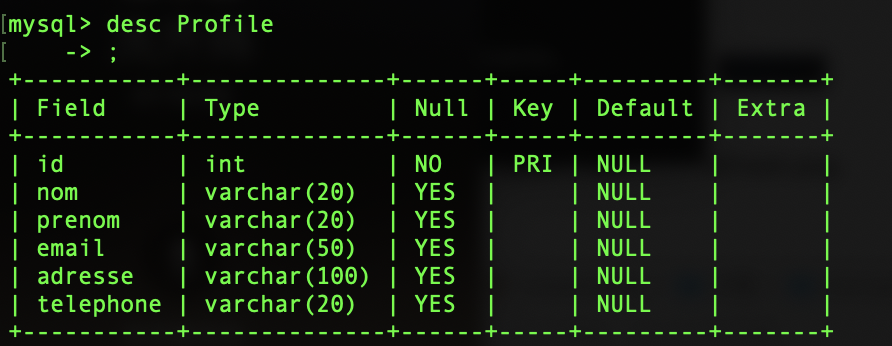
\includegraphics[width=0.5\textwidth]{tableProfile.png}\\
				\caption cf.tableProfile
			\end{minipage}%
		}%
\end{figure}
\begin{figure}
		\subfigure{
			\begin{minipage}[t]{\linewidth}
				\centering
				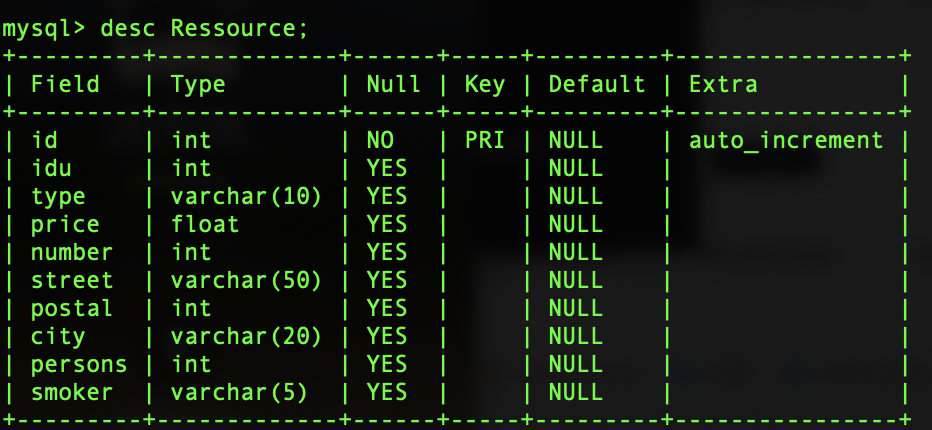
\includegraphics[width=0.5\textwidth]{tableRessource.png}\\
				\caption cf.tableRessource
			\end{minipage}%
		}%
\end{figure}
\begin{figure}
		\subfigure{
			\begin{minipage}[t]{\linewidth}
				\centering
				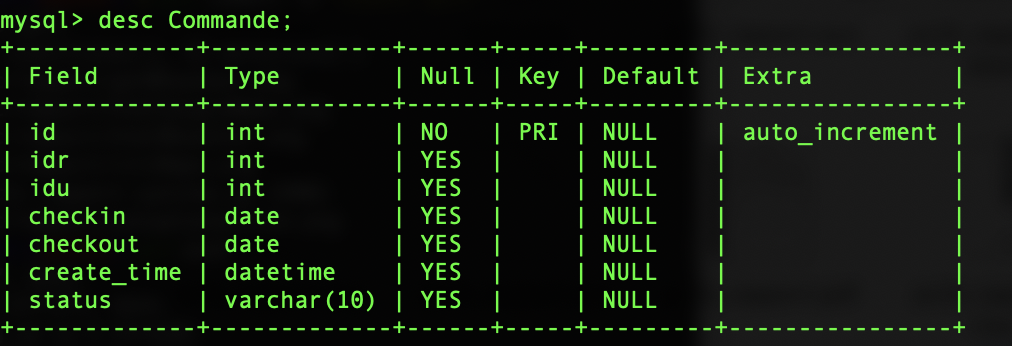
\includegraphics[width=0.5\textwidth]{tableCommande.png}\\
				\caption cf.tableCommande
			\end{minipage}%
		}%
\end{figure}





\section{Structure du serveur}

\section{Structure du client}

\section{Requêtes et réponse}

\section{Conclusion}

\section{Annexe}
\begin{figure}
		\subfigure{
			\begin{minipage}[t]{\linewidth}
				\centering
				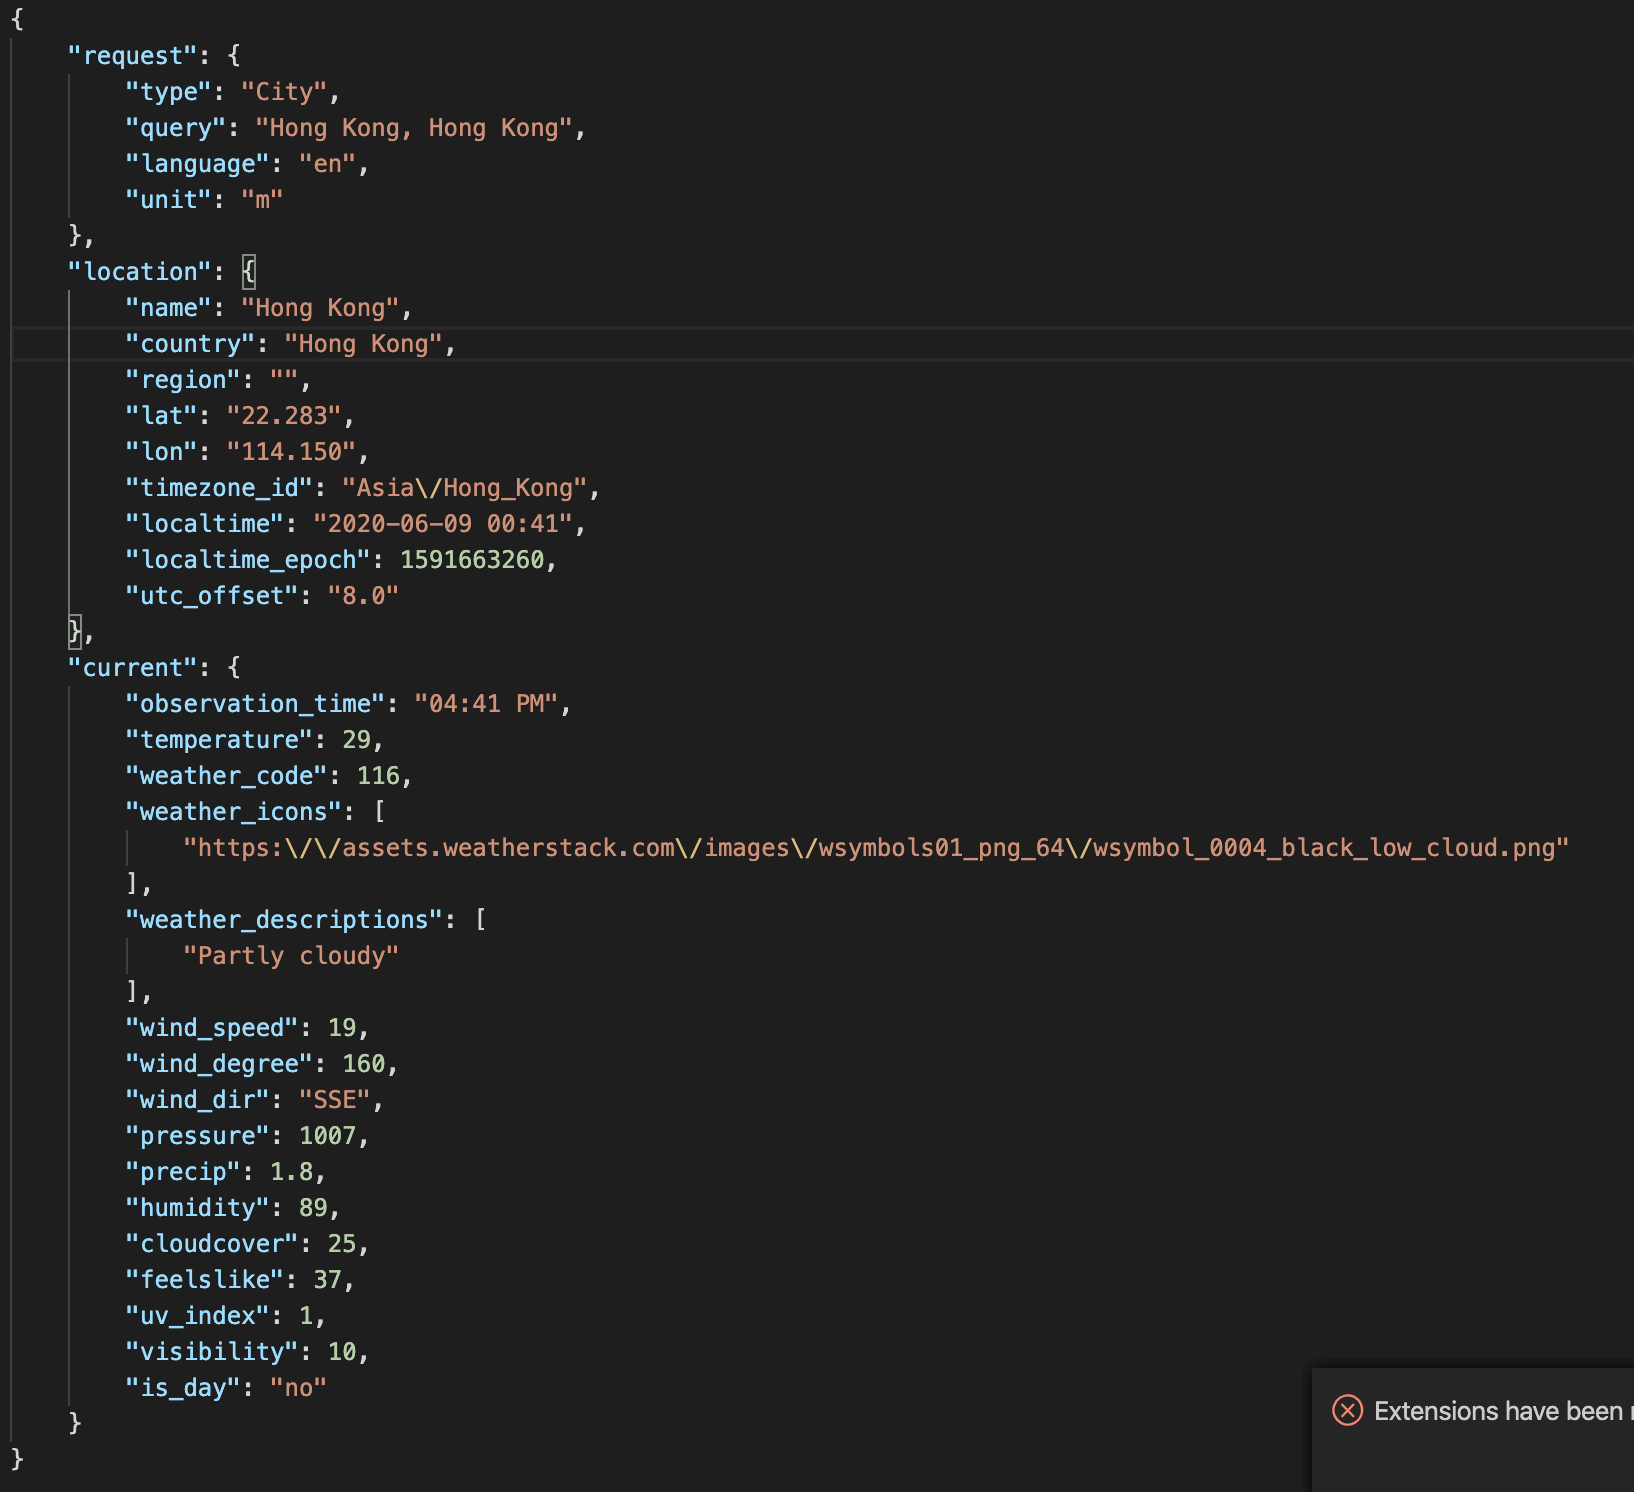
\includegraphics[width=0.8\textwidth]{json.png}\\
				\caption cf.Données Json
			\end{minipage}%
		}%
\end{figure}
\section{Référence}
[1]Weatherstack,[Online].Available:https://weatherstack.com/\\

[2]Google Maps,[Onlone].Available:https://cloud.google.com/maps-platform/\\
\end{document}
